 \newpage
 \vskip 6mm
 \pagestyle{myheadings}
 \markboth{{\underline{\centerline{东南大学博士学位论文} }}}
 {{\underline{\centerline{第四章 \ \ \  基于多级小波分解和传递熵的车辙预测框架} }}}
 
 \chapter{基于多级小波分解和传递熵的车辙预测框架}\label{ch4}
 \setcounter{equation}{0}
\section{引言}
在前两章中,我们对以传递熵为基础的因果关系模型进行了理论和方法上的创新。从本章开始,我们将展示基于传递熵的因果网络在复杂系统中建模的应用。以沥青路面车辙预测模型为例,本章将展示因果网络作为模型中特征选取模块的应用。
车辙作为沥青路面的一种主要破坏形式,不仅会导致路面结构性能衰减,还会加速路面损坏。此外,车辙还会威胁行车安全,对正常交通极为不利\cite{1,2}。同时,由于车辙变形既发生在沥青路面的面层,也发生在下层,因此车辙的养护工作十分困难\cite{3}。车辙问题的解决不仅有赖于抗车辙材料的研发和沥青路面抗车辙性能的提高,还可以在设计阶段根据路面的影响因素预测车辙变形的发展,从源头上保证路面的抗车辙性能\cite{4}。因此,高精度车辙预测模型的研究对于评价车辙病害、提高路面使用寿命具有重要意义。
近年来,车辙预测研究取得了长足的发展。然而,以下两个突出问题依然存在,并严重制约了车辙预测性能及其应用。第一个问题是缺乏有效的、通用的数据处理、特征选择和建模框架。车辙预测模型的研究需要分析车辙变形的影响因素,车辙变形是沥青路面在交通荷载因素、气候环境因素和路面材料因素的耦合作用下产生的永久变形。常见的经验模型是基于多元回归分析,这种方法会忽略历史数据的依赖性。因此,时间序列模型通常用于研究复杂系统并了解其随时间变化的行为方式(cite{5})。从统计学角度来看,时间序列模型的一般定义可表述为:
\begin{eqnarray}
\hat{y}_{i,t+n} = f(Y_{i,t-k},X_{j,t-k},s), \nonumber
\end{eqnarray}
其中,模型输出 $\hat{y}_{i,t+n}$ 为序列,$n$ 为预测步数;$Y_{t-k}=\{y_{t},y_{t-1},...,y_{t-k}\}$ 是 $\hat{y}$ 的历史数据;$i$ 是前提条件维度,在本任务中等于 1;$X_{j,t-k}=\{x_{j,t},x_{j,t-1},...,x_{j,t-k}\}$是输入变量序列,$j$代表输入维度;$s$是与实体相关的静态信息。上述三项构成了模型的整个输入,而 $f: R^{i\times k}\rightarrow R^{m}$是待确定的预测模型。随着统计学和大数据的发展,基于机器学习和深度学习的车辙预测模型已被引入,有助于实现长期时间序列建模\cite{6}。特别地,作为复杂系统数据处理的常用技术,时间序列分解通常用于识别原始时间序列的趋势分量和波动分量\cite{7}。此外,基于因果关系的特征值对于建立可解释且稳健的预测模型也有潜在的益处 \cite{5}。


第二个问题是缺乏可信的沥青路面数据。沥青路面的数据来源主要包括:实验室试验、加速路面试验(APT)、路面长期性能跟踪(LTPP)等。与实验室试验和 LTPP 研究相比,加速路面试验不仅能更真实地反映路面的使用状态,而且能在更短的时间内获得路面的使用状态数据。因此,全尺寸轨迹作为一种收集多种路面结构和材料时空性能数据的典型 APT 方法,已被许多国家的研究机构和研究人员广泛采用。交通运输部公路科学研究院轨道(RIOHTrack)是我国第一条全尺寸轨道,于2017年在北京建成\cite{9}。
为克服上述问题,本文提出了一种基于小波分解和多元转移熵的新型车辙预测框架,旨在以可解释的分析方法捕捉车辙及其影响因素之间的因果关系,准确预测车辙演变曲线。本文提出的框架包括三个模块:基于多级离散小波分解(MDWD)的数据处理模块、基于多元传递熵(MTE)的特征选择模块和基于机器学习模型的预测模块。在车辙预测模块中,使用了两个预测模型进行车辙预测,分别是用于预测高频分量的多元高斯过程回归模型(GPR)和用于预测低频分量的双向门控循环单元(bi-GRU),并进一步提供了基于这两个模块的一些因果关系分析。最后,预测结果通过反小波变换进行重构,将各频段的预测结果融合为框架的输出结果。性能比较结果表明,所提出的框架比一些最先进的基线时间序列预测模型更有效。此外,本章还设置了消融实验,以评估每个模块对框架性能的影响。

\section{相关工作}
\subsection{车辙预测模型}
沥青路面车辙评价机理可分为三个阶段\cite{10}。第一阶段是初始沥青混合料的压实过程。该阶段的车辙是人工为提高路面承载能力而产生的。第二阶段为稳定阶段,车辙是沥青混合料在高温或重载作用下抗剪能力不足而产生的流动变形。两侧的隆起量逐渐与凹陷量相等。这一阶段车辙演变的速度相对较慢。第三阶段为快速发展阶段,沥青混合料骨架结构的重新排列过程和沥青混合料的剪切破坏是车辙产生的主要原因。在这一阶段,车辙加深的速度明显加快。从以上分析可以看出,沥青路面车辙主要是沥青层在外部环境因素和内部结构因素的双重作用下产生的流动变形\cite{11,12}。
近年来,人们在车辙预测模型方面做了大量工作。车辙预测模型可分为三类:力学模型、经验模型和力学-经验模型。力学模型以弹性或粘弹性-塑性分层体系理论为基础,通过分析材料变形与应力、应变之间的关系来预测沥青路面的车辙深度。\cite{13}根据实验室蠕变试验的结果提出了修正的麦克斯韦模型。\cite{14}提出了带有时间和温度因子的臼化 Burgers 模型。cite{15}利用统计学原理分析了车辙与其他影响因素之间的关系,并在此基础上建立了预测车辙的经验模型。\cite{16}提出了车辙预测模型,并分析了多变量影响因素。引入了一些深度学习模型以提高车辙预测模型的准确性。\cite{17}提出了基于多层感知(MLP)的车辙演变模型。力学-经验模型基于力学理论建立车辙预测模型,并通过实词数据计算参数。其代表作是 AASTO2002 模型,该模型提供了一种称为 MEPDG 的模型设计方法,用于建立各层的车辙预测模型。M-E模型的参数训练可以采用多元线性回归(MLR)和随机预测的方法,这样可以提高50\%的精度\cite{19}。

\subsection{路面材料和结构的非稳态时间序列预测}
实践中的复杂系统往往表现出多变量非稳态演化行为,所获得的系统信息通常是不完整和不确定的。一般来说,对于沥青路面车辙演变预测这样的典型复杂任务,很难建立精确的分析数学模型。因此,通常通过观测或实验获取时间序列来分析复杂系统。非平稳时间序列预测旨在分析多变量之间的关系,了解纵向观测数据的依赖性,历来是学术界研究的热门领域,应用广泛。从广义上讲,非平稳时间序列的预测模型可分为参数模型和非参数模型,这取决于模型是采取预定义的形式还是纯粹由数据驱动的构造\cite{20}。

参数预测模型通常提供一个具有有限数量参数 $\theta$ 的显式函数来描述输入 $X$ 和输出 $Y$ 之间的关系,其中 $\theta$ 是通过时间序列变现来优化的\cite{21}。作为静态时间序列的经典自回归模型,ARIMA 通过差分来降低非静态性。\cite{22}使用基于 ARMIA 的模型,通过建立结构时间序列来预测交通基础设施。基于神经网络和深度学习的方法因其强大的拟合能力和无需静态假设而被广泛应用于非静态时间序列预测任务中。本文提出了一种基于特征融合 LSTM-BPNN 的路面性能预测模型,并引入了注意力机制 \cite{23}。基于支持向量机(SVM)的模型是另一种经典的参数模型,例如,\cite{24}提出了一种基于粒子群优化(particle swarm optimization,PSO)和支持向量回归(support vector regression,SVR)的沥青路面性能预测模型。

与参数模型相比,非参数模型是在大量观测数据的基础上表示非平稳的动态变化,不需要结构假设和复杂的建模。\cite{20}和\ cite{25}在路面裂缝问题上测试并比较了多种非参数机器学习方法,包括随机森林、朴素贝叶斯和 K-近邻算法。\cite{26} 将经验模态分解(empirical mode decomposition,EMD)引入路面裂缝分析。\cite{27}使用小波分解处理车辙深度时间序列数据,并用ARIMA预测车辙,该方法可以捕捉时间序列的频率特性进行车辙预测。

  
\section{模型描述}
本章提出的多元时间序列分析方法可分为三个模块:(1)基于多级小波分解(MDWD)的数据处理;(2)基于多元传递熵(MTE)的因果推断;(3)混合时间序列预测模型。该方法的架构如图\ref{fig4_1} 所示,其中 MDWD 模块和 MTE 模块在框架的多尺度因果特征检测中发挥了重要作用。基于 MDWD 模块,原始时间序列被分解为低频分量和高频分量,分别代表原始时间序列的趋势项和波动项。然后,MTE 模块选择与车辙具有显著静态偶然关系的影响因素作为各频段时间序列预测模型的特征。最后,对各频段的预测序列进行重构,设计基于融合注意力机制的预测模型,生成车辙预测结果。本节接下来将详细介绍这三个模块。

\begin{figure*}[ht]
\begin{center}
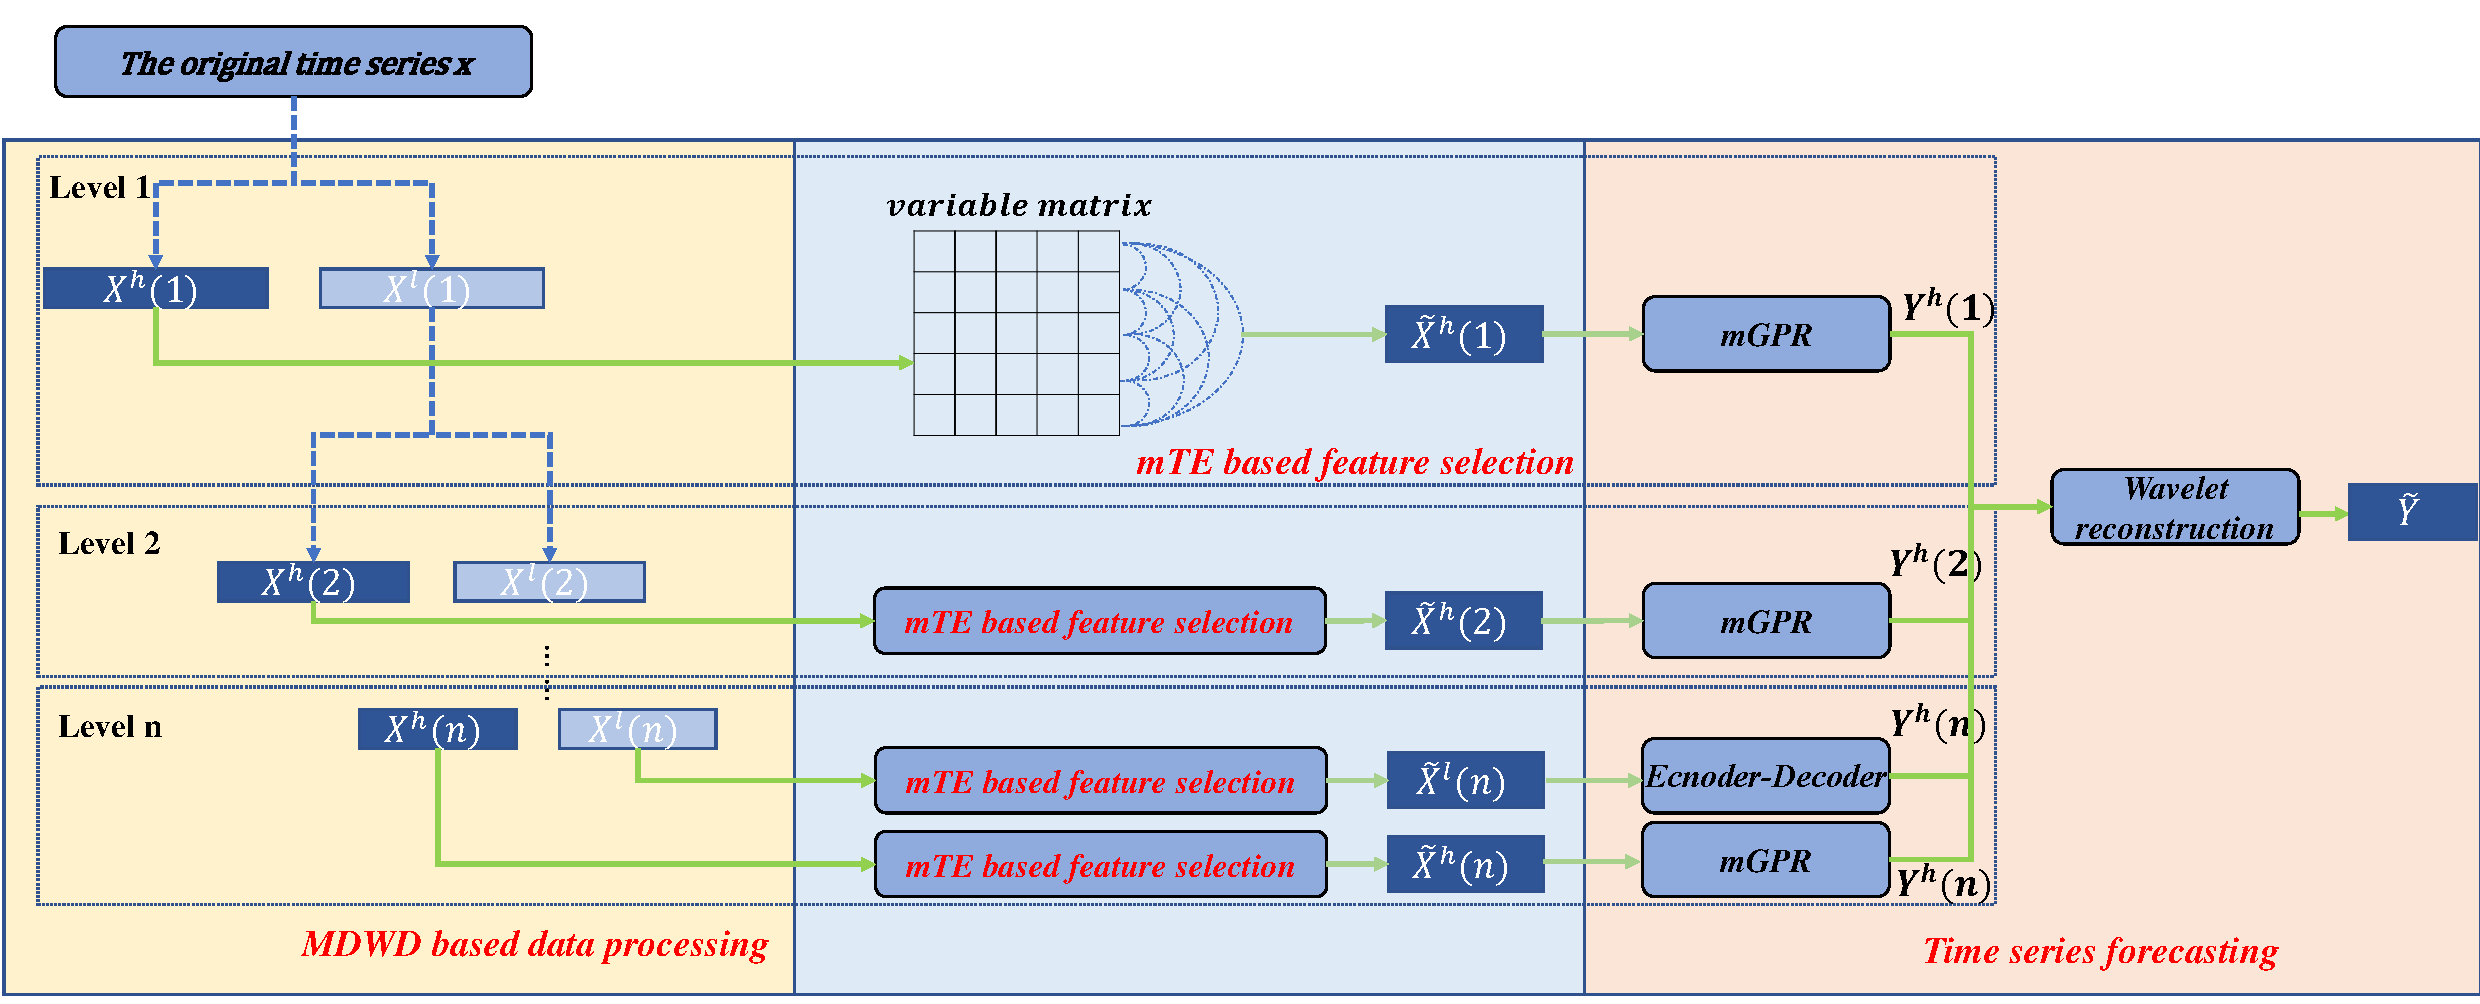
\includegraphics[scale=0.4]{./ch4/fig4_1.pdf}
\caption{基于多级小波分解和多元传递熵的时间序列分析框架示意图} \label{fig4_1}
\end{center}
\end{figure*}
所提模型的结构包括三个模块:基于 MDWD 的数据处理模块、基于 MTE 的特征选择模块和时间序列预测模块。模型的输入$X \in \mathbb{R}^{n\times T}$由$n-1$个影响因素和长度为$T$的车辙时间序列组成。输出$\tilde{Y}\in\mathbb{R}^{1\times \tau}$为沥青路面车辙预测值,其中$\tau$为预测步长。基于 MDWD 的数据处理模块将输入分解成不同的层次。每一级中的高频成分和最后一级中的低频成分作为每一级中相应的基于 MTE 的特征选择模块的输入。最后,在时间序列预测模块中,高频成分预测模型采用多元高斯过程回归模型,低频成分预测模型采用基于双向长短记忆网络(LSTM)和融合注意力机制的预测模型。

\textbf{基于 MDWD 的数据处理模块} 有关多级小波分解(MDWD)概念介绍及推导已在第二章中给出,本章不再赘述,这里只给出本章所提出框架中使用的内容。其中MDWD模块分为时间序列分解部分和重构部分,对于分解部分,给定输入时间序列 $X_{t}=x_{1},x_{2},...,x_{t}$,MDWD 在 $(i+1)$-th 层的分解输出可定义为:

\begin{equation}\label{npl1}
\begin{array}{ll}
y^{l}_{t}(i+1) = \sum_{k=1}^{K}x^{l}_{t+k-1}(i)\cdot l_{k},\\
\\
y^{h}_{t}(i+1) = \sum_{k=1}^{K}x^{l}_{t+k-1}(i)\cdot h_{k},\\
\end{array}
\end{equation}

其中,右侧的输入为第 i 层的低频序列分量 $X^{l}$ 和高频序列分量 $X^{h}$,它们是是上一层分解的子序列 $Y^{l}$ 和 $Y_{h}$ 的下采样,输出$y^{l}_{t}(i+1)$ 和$y^{h}_{t}(i+1)$ 分别是 $t$ 时间步长的低频序列分量和 $i$ 级别的高频序列分量。函数 $l_{k}$ 和 $h_{k}$ 是低通和高通滤波器的脉冲响应。从每一层的低频分量 $Y^{l}$ 和高频分量 $Y_{h}$可以重建级别 $i-1$ 的时间序列 $X$:	
\begin{equation}\label{npl1}
\begin{array}{ll}
x^{l}_{t}(i-1) = \sum_{k=1}^{K}y^{l}_{t+k-1}(i)\cdot l_{k}+\sum_{k=1}^{K}y^{h}_{t+k-1}(i)\cdot h_{k}.\\
\\
\end{array}
\end{equation}

这一过程也被称为逆离散小波变换(inverse discrete wavelet transform,IDWT)。它的过程包括向上采样和重建。变换函数 $l_{k}$ 和 $h_{k}$ 是上一级函数的缩放和移位。

\textbf{基于 MTE 的特征抽取模块} 在上一章中,我们已经介绍了一种新型的基于核函数估计的方法来计算MTE,尽管该方法具有准确性高和计算代价小的优点。但由于其本身对于MTE中参数马尔可夫阶数$\tau$的选取并没有针对性的讨论,导致在选取$\tau$值时只能根据经验选择,会出现虚假因果关系,甚至无法发现显著因果关系。为了能够选择出统计显著的传递熵(effective transfer entropy, ETE),本章将继续介绍一种基于贪心算法的MTE计算方法,进一步确定公式中的Markov阶数,首先,我们回顾TE的定义,从 $Y$ 到 $X$ 的 TE 是以历史数据 $X_{t}^{k}$ 为条件,从源过程 $Y_{t}$ 到 $X$ 的实现值 $x_{\tau}$ 的条件互信息:
\begin{equation}\label{TE}
\begin{array}{ll}
T_{Y\rightarrow X}=I(Y_{t}^{k};x_{\tau} |X_{t}^{k})=-\sum^{t-k}_{i=1}\frac{log(p(x_{\tau}|x_{i},y{i}))}{p(p(x_{\tau}|x_{i}))},
\end{array}
\end{equation}
其中$Y_{t}^{k}$和$X_{t}^{k}$为长度为$k$的历史序列,$x_{\tau}$为$\tau$时刻的随机变量。$T_{Y\rightarrow X}$大于0意味着$Y$是$X$的原因。否则,$Y$就是$X$的结果。值得注意的是,TE取决于历史序列长度$k$。$T_{Y\rightarrow X}$可以表示整个概念信息传递,而$k\rightarrow \infty$。但是,$\tau$值的选取会影响TE的显著性,甚至会带来冗余信息。为了克服这些问题,\cite{31}提出了集体传递熵(CTE),它表示因果源的增量条件互信息之和:
\begin{equation}\label{npl1}
\begin{array}{ll}
T_{Y\rightarrow X}=\sum\limits_{G} I(z_{n},t;y_{t+\tau}|y_{t}^{k},z^{<n}),
\end{array}
\end{equation}
其中 $z^{<n} \in Z$ 中的 $z^{<n}$ 是额外的源变量集,用于检测来自 $X$ 的冗余变量:${z^{<n}}=\{Z_{c}|\forall c: 1\leq c \leq n\}$。受 \cite{32} 的启发,我们提供了一种贪婪算法,根据 CMI 对候选变量 $C$ 的贡献从 $X$ 中选择 $Z$。算法如算法 1 所示:

\begin{algorithm}[htb]
\caption{基于贪心算法的有效传递熵(ETE)的计算}
\label{alg:SA1}
\hspace*{0.02in} {\bf 输入:} 多元源时间序列 $X$, 目标时间序列 $Y$, 相关源序列集 $Z$ 和变量历史数据候选集 $C_{X}$ and $C_{Y}$.\\
\hspace*{0.02in} {\bf 输出:} 多元因果关系集 $E$.\\
\begin{algorithmic}[1]
%\ENSURE ~~Split data set into $k$ folds $F:\{F_{1}, F_{2},..., F_{k}\}$\
\STATE Initialise $\ Z=\emptyset$,  $\ E=\emptyset$
\\

\FOR{$c \in C_{X}$}
    \STATE $T_{c\rightarrow y_{t+ \tau}} = I(c,y_{t}|Z)$;
    \IF {$T_{c\rightarrow y_{t+ \tau}}$ meets $Maximum\ Statistics$}
        \STATE add $c$ to $Z$ and remove it from $C_{Y}$;
    \ELSE
        \STATE break;
    \ENDIF
\ENDFOR
\FOR{$c' \in C_{Y}$}
    \STATE $T_{c\rightarrow y_{t+ \tau}} = I(c',y_{t}|Z)$;
    \IF {$T_{c\rightarrow y_{t+ \tau}}$ meets $Maximum\ Statistics$}
        \STATE add $c'$ to $Z$ and remove it from $C_{X}$;
    \ELSE
        \STATE break;
    \ENDIF
\ENDFOR
\FOR{$z \in Z$}
    \STATE add $z$ to $Z'$;
    \STATE $T_{z\rightarrow y_{t+ \tau}} = I(Z_{X},y_{t}|Z_{Y})$;
    \IF {$T_{z\rightarrow y_{t+ \tau}}$ meets $Minimum\ Statistics$}
        \STATE remove $z$ from $Z$
    \ENDIF
\ENDFOR
\STATE $T_{Z_{X}\rightarrow y_{t+ \tau}} = I(Z_{X},y_{t}|Z_{Y})$;
\IF {$T_{Z_{X}\rightarrow y_{t+ \tau}}$ meets $omnibus \ test$}
    \STATE add $Z_{X}$ to $E$
\ENDIF
\RETURN $E$
\end{algorithmic}
\end{algorithm}


\subsection{时序预测模型框架}
在小波分解模块中,车辙及其影响因素的时间序列被分解为 3 层,其中最后一层的低频分量(0-20Hz)表示原始时间序列的趋势项,所有 3 层的高频分量(20-30Hz、30-50Hz 和 50-100Hz)表示原始时间序列的波动项。作为递归神经网络(RNN)的扩展,LSTM能够捕捉时间序列的长期依赖关系,而注意力机制的概念在近几年的深度学习,特别是神经网络领域的研究中得到了普及,它能有效捕捉输入数据不同部分之间的依赖关系,这在许多任务中都至关重要。(\cite{33}),因此也被被用于时间序列预测。因此,我们设计了一种基于融合注意力机制和LSTM的自编码器为趋势项的预测模型。此外,为了克服 RNN 模型在面对时间序列高频波动时的不敏感性,本文将基于统计理论的复杂时间序列高维非线性机器学习模型 GPR 引入到所提出的框架中,以预测波动项。本节的其余部分将介绍这两个模型的机制。

\subsection{高斯随机过程} 高斯过程是随机变量的集合,其中任意有限个变量都具有联合高斯分布。给定一组点 $X = \{x_1,x_2,\ldots,x_t\}$,其值 $f(X)$ 完全由其均值函数 $m(X)$ 和协方差函数 $k(X,X')$指定,它们分别定义为:
\begin{equation}
\begin{aligned}
m(X)=\mathbb{E}[f(X)&], \\
k(X,X')=\mathbb{E}[(f(X)-m(X)&)(f(X')-m(X'))],
\end{aligned}
\end{equation}
其中,$f(X)$ 是高斯过程,可写成:
\begin{equation}
\begin{aligned}
f(X) \sim \mathcal{GP}(m(X), k(X,X')).
\end{aligned}
\end{equation}

用 $y$ 表示观测值,它与真实值 $f(X)$ 之间存在加性噪声。我们假设噪声服从独立、同分布的高斯分布,均值为零,方差为 $\sigma^2$:
$$\varepsilon \sim \mathcal{N}(0,\sigma^2).$$

根据 $f(X)$ 和先验分布,可以推断出在一组点 X 上产生的真值的期望值和方差。具体来说,要根据已知观测值和先验值估计真值 $f(X)$,我们需要联合分布:
\begin{equation}
\left[\begin{array}{c}
\boldsymbol{y} \\
\boldsymbol{f}^{\prime}
\end{array}\right] \sim \mathcal{N}\left(\left[\begin{array}{c}
\boldsymbol{\mu} \\
\boldsymbol{\mu}^{\prime}
\end{array}\right],\left[\begin{array}{cc}
\boldsymbol{K}(X, X)+\sigma_{n}^{2} I & \boldsymbol{K}\left(X^{\prime}, X\right) \\
\boldsymbol{K}\left(X, X^{\prime}\right) & \boldsymbol{K}\left(X^{\prime}, X^{\prime}\right)
\end{array}\right]\right),
\end{equation}

以及观测数据的联合高斯先验分布

\begin{equation}
\begin{aligned}
P(f'\mid y,X,X')=\mathcal{N}(m,C).
\end{aligned}
\end{equation}

有一些常用的协方差矩阵函数 K,通过对数似然框架中的优化,可以自适应地获得最佳超参数。函数值 $f'$(对应于测试输入 $X'$)可以通过评估点 $X$ 的估计均值 m 和估计方差 $C$ 从联合后验分布中采样:
\begin{equation}
\begin{array}{c}
\boldsymbol{m}=\boldsymbol{\mu}^{\prime}+\boldsymbol{K}\left(X, X^{\prime}\right)\left(\boldsymbol{K}(X, X)+\sigma_{n}^{2} I\right)^{-1}(\boldsymbol{y}-\boldsymbol{\mu}) \\
\boldsymbol{C}=\boldsymbol{K}\left(X^{\prime}, X^{\prime}\right)-\boldsymbol{K}\left(X, X^{\prime}\right)\left(\boldsymbol{K}(X, X)+\sigma_{n}^{2} I\right)^{-1} \boldsymbol{K}\left(X^{\prime}, X\right)
\end{array}
\end{equation}

\subsection{基于融合注意力机制的自编码器}
本节所提出的时间序列预测模型利用了长短期记忆和融合注意力机制,是一个端到端的深度学习框架,它将编码上下文向量和注意力向量相互融合,从而进行时间序列表示学习。模型架构见图\ref{fig4_2}。模型的流程如下:在经过特征提取后的序列$X_{n}=\{x_{1}, x_{2}, ... ,x_{n}\}$被当模型输入送入编码器模块,首先进入LSTM模型,生成隐向量$h_{t}$,作为注意力层的输入。注意力层包括两种注意力机制:自注意力(self-attention)和时间注意力(temproal attention),图中$h'_{t}$表示自注意层在时间步长为t时的输出向量,其维度为$l$,滑动窗口大小为t。在时间注意力层中有t个1维 CNN 滤波器$C_{i}$,($i \in l$),其大小为$t\times 1$。通过滤波器对$h'_{t}$进行卷积,产生一组行向量 $H^{C}$,其大小为 $k \times l$)。接下来,关注度权重 $\alpha_{i}$,($i \in l$),即行向量中元素相关性,由评分函数 $f: \mathbb{R}^{k \times l} \times \mathbb{R}^{l}\mapsto \mathbb{R}$。最后,编码器的输出向量 $\tilde{h}^{'}_{t}$ 是由 $h^{'}_{t}$ 和原始向量 $h_{t}$ 连接生成的。在本节的剩下部分,我们将详细介绍模型内所涉及到的模块。

\begin{figure*}[ht]
\begin{center}
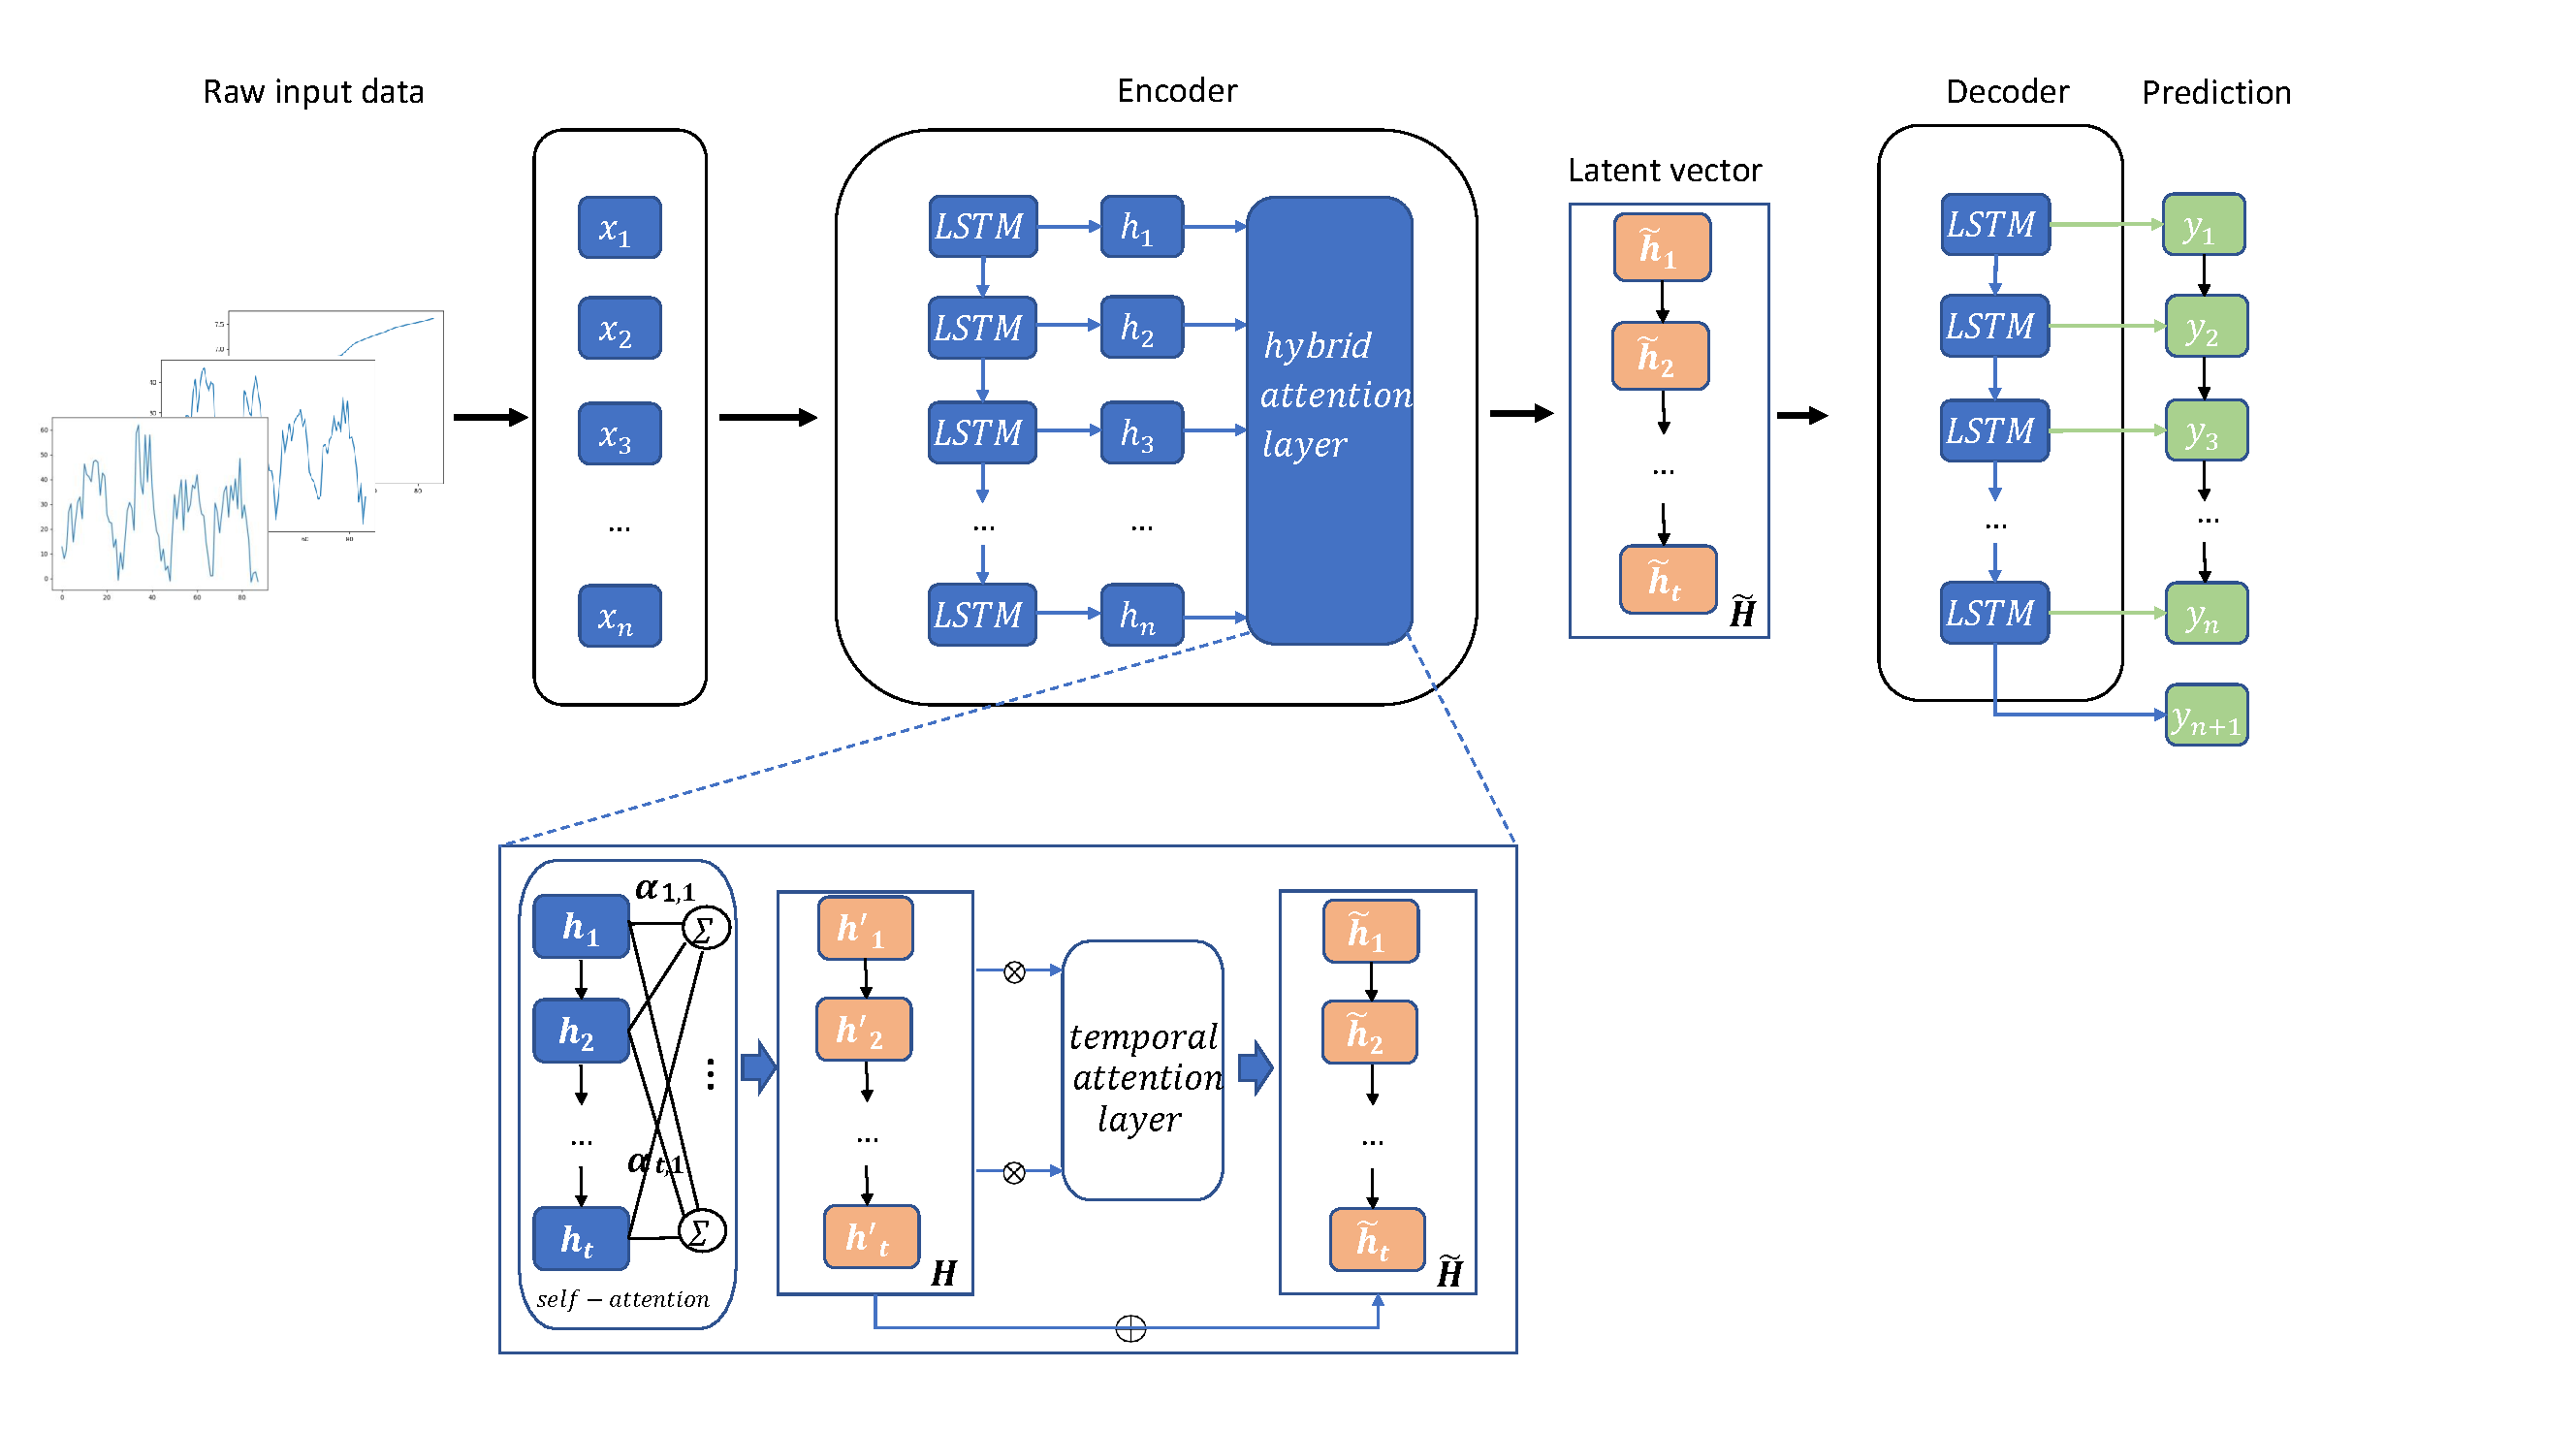
\includegraphics[scale=0.4]{./ch4/fig4_2.pdf}
\caption{基于融合注意力机制的自编码器} \label{fig4_2}
\end{center}
\end{figure*}

\textbf{长短记忆网络} 长短记忆网络(long short term memory, LSTM)是 Hochreiter 等人提出的 RNN 变体\cite{SHochreiter1997}。LSTM 继承了循环神经网络(recurrent neural network,RNN)对时间序列数据的上下文信息进行动态建模的能力,还能处理不同长度和维度的变量序列。通过引入门机制,LSTM 克服了RNN在长期序列依赖问题和梯度消失问题。为了解决这些问题,LSTM 使用单元状态 $c_{t} $中存储长期信息,并在隐藏状态 $h_{t}$来处理当前信息:

\begin{eqnarray}
&& h_{t} = o_{t}\odot \tanh(c_{t}),\\
&& o_{t} = \delta(W_{x_{o}}x_{t}+W_{h_{o}}h_{t-1}),\\
&& c_{t} = {f}_{t}\odot {c}_{t-1}+i_{t}\odot \tanh(W_{x_{g}}x_{t}+W_{h_{g}}h_{t-1}),\\
&& i_{t} = \delta(W_{x_{i}}x_{t}+W_{h_{i}}h_{t-1}),\\
&& f_{t} = \delta(W_{x_{f}}x_{t}+W_{h_{f}}h_{t-1}),
\end{eqnarray}

其中,$i_{t}$, $f_{t}$, $o_{t}$ 分别是输入门、遗忘门和输出门,$W_{x_{i}}$, $W_{x_{f}}$, $W_{x_{o}}$, $W_{x_{g}} \in \mathbb{R}^{m\times i}$ 是每个门控的可学习参数矩阵。编码器中的 LSTM 层用于将多变量输入编码为隐藏状态 $H_{t}=\{h_{1}, h_{2}, ... , h{t}\}$ ,这是一个固定大小的向量,作为混合注意力层的输入。而输出的大小$Y_{t}=\{y_{1},y_{2}, ... ,y_{t}\}$ 由解码器中的 LSTM 生成,长度可以按需指定。

\textbf{注意力机制} 注意力机制模拟了认知心理学中引入的人脑注意力。注意力机制的发展也引领了长期时间序列依赖性学习。本节引入了两种注意力机制,首先介绍自注意力机制,自我注意力的提出是为了克服序列生成的变换器架构中的一个问题,即固定大小的嵌入引起的信息损失\cite{AVaswani2017}。注意力层将每个时间步的时间信息与动态生成的注意力值聚合在一起,这样模型就能锁定重要的时间步,并消除长期序列中的无用信息。从概念上讲,注意力是一种基于给定查询的键值查找机制,可表述为:
\begin{eqnarray}
&& h_{t} = \sum^{T}_{\tau = 0} \alpha (q_{\tau},k_{t})v_{t-\tau },\\
&& \alpha (q_{\tau},k_{t}) = exp(\frac{q_{\tau} \cdot k_{t}^{T}}{\sqrt{d_{k}}}) \// \sum^{T}_{\tau = 0} exp(\frac{q_{\tau} \cdot k_{t}^{T}}{\sqrt{d_{k}}}),
\end{eqnarray}
其中,$H_{t}$ 是自注意力机制的输出;$Q_{\tau}$、$K_{t}$ 和 $v_{t-\tau}$ 是输入线性变换的中间矩阵,$Q、K$ 和 $V$ 在不同时间步的特征向量表示;$\alpha$ 是可学习的自注意系数。自注意力机制的第一步是对输入特征 $x_{\tau}$ 和输出状态 $h_{t}$ 进行相似度测量。相似度越高,输入的注意力就越强。上式中的相似度运算是向量点积,也可以用余弦相似度或输入 $h_{t}$ 和输出 $\alpha_{t}$ 的多层感知器(MLP)来代替。第二步是加权平均算子,用于消除量纲影响\cite{AVaswani2017}。

自注意力主要集中在描述每个连续隐藏向量元素在时间维度的重要性上,这种设计忽略了行元素对输出包含信息的影响,尤其是在多变量任务中,它无法检测到有用的时态模式。而隐向量的行元素之间的关系则可以时间注意力来捕捉,时间注意力的具体架构如图\ref{fig4_3} 所示。给定回视窗口 $t$ 中的 RNN 单元隐藏状态矩阵 $H_{t-1} \in \mathbb{R}^{m\times t}$,时态模式关注机制关注用 $K$个1维的CNN 过滤器 $C_{i}\in \mathbb{R}^{t\times 1}$ 操作每个向量 $h$ 中的行元素,所有向量得到的结果组成矩阵 $H^{C} \in \mathbb{R}^{l\times k}$。最后,使用评分函数 $f: \mathbb{R}^{l\times k}\longmapsto \mathbb{R} $ 来计算矩阵 $H^{C}$ 和隐藏状态 $h_{t}$ 在时间步长 $t$ 中的相关性,因此时间注意力可以表述为:
\begin{eqnarray}
&& \hat{h}_{t} = W_{h^{'}}h^{'}_{t}+W_{h}h_{t},\\
&& h^{'}_{t} = \sum^n_{i=1}\alpha_{i}\widetilde{H}^{C}_{i},\\
&& \alpha_{i} = \frac{exp(f(\widetilde{H}^{C}_{i},h_{t}))}{\sum^{n}_{i=1} exp(f(\widetilde{H}^{C}_{i},h_{t}))},\\
&& f(\widetilde{H}^{C}_{i},h_{t}) = (\widetilde{H}_{i}^{C})^{\top}W_{a}h_{t},\\
&& \widetilde{H}_{i,j}^{C} = \sum^{K}_{j = 1} r_{j} \times C_{i},
\end{eqnarray}


\begin{figure}[htbp]
\begin{center}
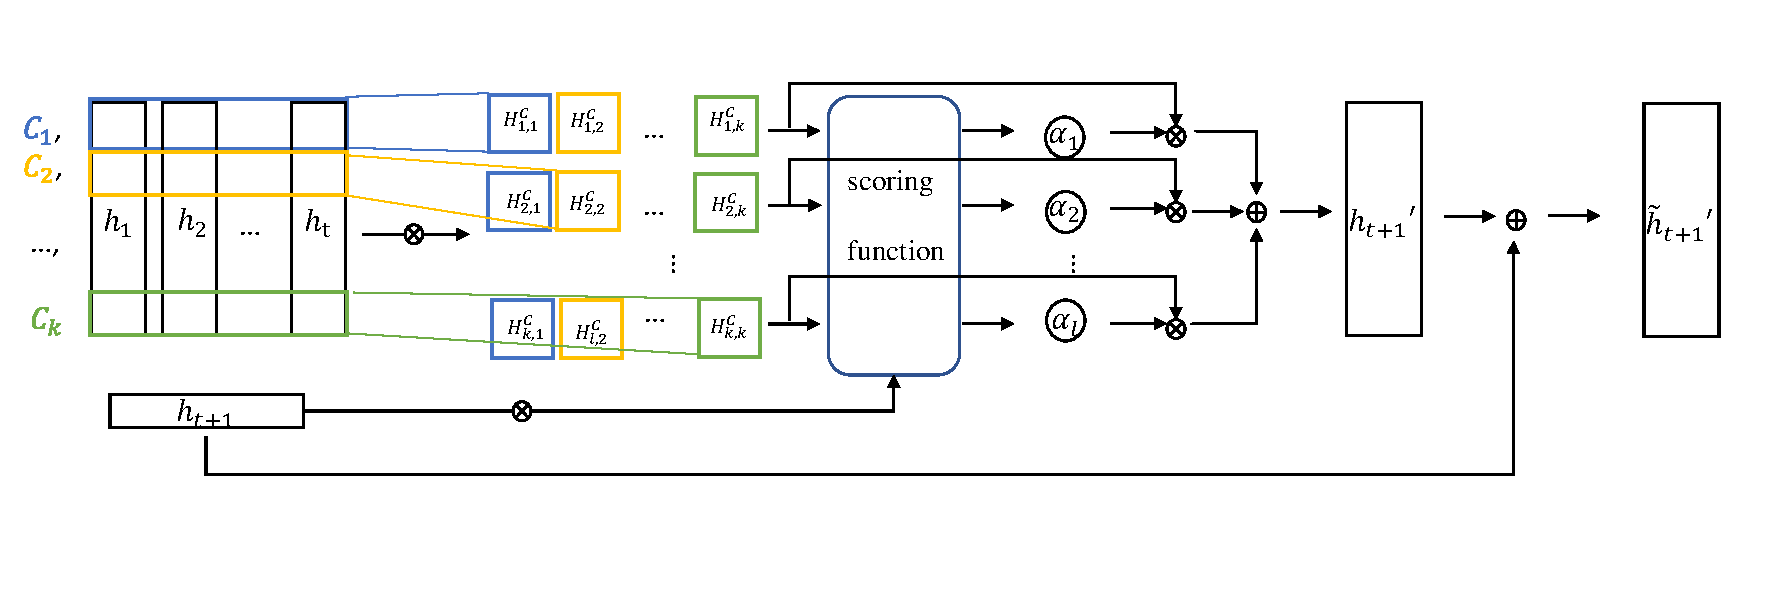
\includegraphics[scale=0.4]{./ch4/fig4_3.pdf}
\caption{时间模式注意力原理图。}\label{fig4_3}
\label{fig2}
\end{center}
\end{figure}
其中,$h^{'}_{t}$ 是时间注意力机制的输出矩阵,$h_{t}$ 是上一步LSTM的输出矩阵,$W_{h^{'}}$,$W_{h}$ 分别是对应的参数矩阵;$\alpha_{i}$ 是 $H_{t}$ 中 $i$ 行元素的注意力权重,由式(4.3.19)中的评分函数 $f$ 计算得出;式(4.3.20)中的$\widetilde{H}^{C}$ 表示卷积运算的权重;$r_{j}$ 是 RNN 单元的输出矩阵,$W_{h^{'}}$,$W_{h}$ 分别是参数矩阵。评分矩阵中每行的权重可以代表行元素与输出 $h'_{t}$ 之间的相关性。


\section{实例结果及讨论}\label{ne}
为了验证本章所提出的时间序列预测框架的有效性,采用RIOHTrack数据集作为实例并设计验证实验。实例结果包括三个部分:时间序列分解模块中小波基函数的选择;特征选择模块中有效传递熵的结果验证;以及预测模型的性能分析及对比。
\subsection{小波基函数的选择}
车辙序列进行小波变换的目的是提高车辙数据的稳定性。与上一章选择小波基函数的原则相同,主要是根据小波变换后数据的平滑度,具体可量化为以下几个方面:正交性、支持集、规则性和消失矩的阶数。根据上述原则,我们继续从Haar小波、Daubechies小波、 Symlets小波,和Coiflets小波中进行选择,每个小波的最优滤波系数由第二章所提出的自适应算法求得。我们给出两个指标来衡量小波函数的分解性能:1.时间序列的小波重构误差,即重构序列$X'$与原序列$X$的均方误差(mean squre error,MSE):$\rm{MSE}(X,X')$;2.高斯过程验证(Gaussian process validation, GPV),即验证采样时间点中不符合高斯随机过程的点数。此外,对于分解层数,我们继续按照第三章中的经验,设置分解层数为2层。验证结果如表\ref{table1}所示:

\begin{table}
	\centering
	\caption{小波基函数的选择 }
	\begin{tabular}{lllll}
	
		小波基函数& 公式 &MSE& \multicolumn{2}{l}{\begin{tabular}[c]{@{}l@{}}GPV\end{tabular}}   \\
		\hline
		&& & $R^{h1}$ & $R^{h2}$ \\
		\hline
		db4                                                & 369.8 & 5.3 & 3.8            & 14  \\
		\hline
		db20                                                & 369.7 & 5.6 & 3.3            & 10  \\
		\hline
		Symlets4                                              & 370.6 & 5.5 & 3.3            & 11 \\
		\hline
		Symlets20                                               & 369.8 & 5.1 & 3.7            & 9   \\
		\hline
		Coiflets21                                               & 369.6 & 5.3 & 3.6            & 10  \\
		\hline
		Coiflets22                                               & 370.0 & 5.3 & 3.8            & 9  \\
	\end{tabular}
\label{table1}
\end{table}

对于小波基函数筛选的两个指标,$\rm{MSE}(X,X')$的值越小,证明小波分解后的信息损失的越少,小波基函数的性能越好;GPV的值越小,证明分解后的序列更符合高斯分布,越有助于提升GPR预测的性能。同时,考虑到消失矩越大,所需要的计算代价越高。从表\ref{table1}中的结果可知,消失矩越高的的小波基函数,其对应的MSE越小,其中,又以Symlet20小波和Coidlets20小波的MSE最小;同时,无论是第一层高频序列的GPV的Symlets20的GPV。综合以上因素,我们选择Symlets20作为时间序列分解模块的小波基。






\subsection{基于传递熵的因果关系结果验证}

\begin{table}[bp]
    \centering
    \caption{基于转移熵的车辙及其影响因素之间的因果关系,括号中为 $p$ 值,$\rightarrow$ 左侧为源变量及其Markov阶数$l$,$\rightarrow$ 左侧为目标变量及其Markov阶数$k$。}
    \begin{tabular}{llll}
     \hline
      因果关系  & 第一次低频分量 & 第一层高频分量 & 第二层高频分量 \\
      \hline
      温度(3) $\rightarrow$ 车辙(1)& 0.0013 \ (0.8710) & \textbf{0.0792 \ (0.0040)}  & \textbf{0.0812 \ (0.0021)}  \\
      \hline
      荷载(1) $\rightarrow$ 车辙(1) & \textbf{0.1190 \ (0.0003)}  & 0.0036 \ (0.9310)  & 0.0049  \ (0.6711)\\
      \hline
      弯沉深度(5) $\rightarrow$ 车辙(3)&  \textbf{0.0943 \ (0.0000)} & \textbf{0.0596 \ (0.0035)}  &  \textbf{0.0889 \ (0.0014)} \\
      \hline
      弯沉面积(5) $\rightarrow$ 车辙(2) & \textbf{0.1251 \ (0.0002)}  &  \textbf{0.0341 \ (0.0079)} & \textbf{0.0666 \ (0.0061)} \\
      \hline
      车辙(3) $\rightarrow$ 弯沉深度(1) & 0.0091 \ (0.9130)  & 0.0013 \ (0.9005)  & 0.0018 \ (0.9116) \\
      \hline
      车辙(3) $\rightarrow$ 弯沉面积(1) & \textbf{ 0.0875 \ (0.0010) }&  0.0037 \ (0.9375) &  0.0017 \ (0.3671)\\
      \hline
\end{tabular}\label{table2}
\end{table}

我们还比较并显示了每个变量在不同频率下的情况,如图 7 所示。然而,变量之间的相关性并不能直观地发现。为了定量测量不同频段车辙及其影响因素之间的偶然性,本文采用了贪心算法的显著TE计算方法,其中源变量和目标变量候选集的长度均为10。在对所有19种路面数据集进行影响因素与车辙之间的偶然性分析后,结果如表\ref{table2}, 所示,括号内表示转移熵的P值。高亮显示的数据表示该数据具有统计意义。根据公式 ,MTE 的核心思想是:如果一个变量引起另一个变量,那么源变量的历史数据的分布应该为目标变量的未来值提供额外的转移信息,而不是仅仅从目标变量的过去值就能预测到的。因此,从源变量到目标变量的转移熵值越高,因果关系就越强。表\ref{table2}中的结果表明,轴载与车辙的因果关系在低频段(L1)统计显著,这表明轴载主要影响车辙的变化趋势。同时,从温度到车辙的传递熵在统计意义上是显著的。这也表明,在趋势项中,全轮驱动挠度盆面积与车辙的因果关系最强,而在波动项中,温度(H1 层)和全轮驱动中心点挠度与车辙的因果关系最强。} 特别地,在所有频段中,我们都可以观察到车辙与全轮驱动深度和全轮驱动面积之间存在着非常显著的双向信息传递。因此,低频段预测模型选择轴载、全断面深度和全断面面积作为特征,高频段预测模型选择温度、全断面深度和全断面面积作为特征。此外,虽然不同路面的因果关系值不同,但所有路面的偶然关系是相同的。这表明多元转移熵可以在车辙及其影响因素之间建立稳定的因果关系。此外,本章所提出的基于贪心算法的显著TE计算方法,进一步的明确了源变量和目标变量的有效Markov阶数,确定了用于计算的历史长度,可以看到,由本章所提出的方法所计算出的统计显著的因果关系,除了$\rm{TE}(load \rightarrow rutting)$,目标变量和源变量的Markov阶数不是相同的。具体的,以温度和荷载为源变量的因果关系,其源变量的Markov阶数较小,说明其数值变化对车辙的影响较快。以弯沉深度和弯沉面积为源变量的因果关系,其源变量的Markov阶数较大,说明其数值变化对车辙的影响更久。在之后的时间序列预测模块中,这些Markov阶数将作为模型自变量的历史滑动窗口尺寸进行使用。



\subsection{预测模型的性能分析}

为了验证所提出的框架在利用 RIOHTrack 数据集进行车辙预测方面的性能,将其与以下基线时间序列预测模型进行了比较:统计回归模型,包括 GPR 模型和 VARIMA;两个基于深度学习的时间序列预测模型,这两个模型为自编码器,其中的编码器分别由 transformer 模型和双向 LSTM构成,其中滑动窗口大小为 5,层数为 2;transformer模型中的多头注意数为 3,注意力机制为自注意力;解码器中则是一个线性回归模型。所有模型都进行了 1000 次训练。每个路面类别选择一个路面数据作为训练集,其余路面数据作为测试集。在训练集中,80\% 用于训练,20\% 用于验证。

我们使用三个指标来衡量模型的预测性能:平均绝对百分比误差 (MAE)、均方根误差 (RMSE) 和判定系数 $R^{2}$,它们的定义分别是:
\begin{align}
MAPE = &\frac{1}{n}\sum\limits_{i=1}\limits^{n}|\hat{y}_{i}-y_{i}|,\\
RMSE =& \sqrt{\frac{1}{n}\sum\limits_{i=1}\limits^{n}(\hat{y}_{i}-y_{i})^2},\\
R^{2} = &1-\frac{\sum\limits_{i=1}\limits^{n}(\hat{y}_{i}-y_{i})^2}{\sum\limits_{i=1}\limits^{n}(\hat{y}_{i}-\overline{y})},
\end{align}
其中,$y_{t}$ 为时间步长 $t$ 时的车辙地面实况,$\hat{y}$ 为预测值,$\overline{y}$ 为车辙时间序列的真实值。对于 MAPR 和 RMSE,数值越小表示性能越好。$R^{2}$ 的取值范围为 $[0,1]$,该值越接近 1,模型的预测性能越好。$R^{2}$ 的值小于 0 意味着预测值的性能比平均值的性能要差。

在性能对比实验中,我们在来自 RIOHTrack 的 19 种路面车辙数据上比较了所提出的框架和其他先进的时间序列预测模型。预测结果的步长分别为 2、4、8 和 16 步。按照第二章中的聚类结果,我们将路面分为五个簇,结果如表 3、表 4 和表 5 所示。其中,每个路面数据的最佳性能以粗体标出。总体而言,在大多数路面类别的车辙数据上,所提出的框架显然比其他基线模型取得了更好、更稳健的性能。在硬基路面(STR4-5)上的两步预测任务的预测性能最好,其指标为 $MAE=0.97$、$RMSE=1.15$、$R^{2}=0.92$。单向 LSTM 在 STR18-19 的两步预测任务中取得了最佳结果。此外,我们还发现传统的统计方法--多元 GPR 在所有指标上都表现最差。这是因为该模型对预测目标有很强的假设。GPR 和 VARIMA 的 MAE 和 RMSE 值较大,因为这些模型会忽略一些跳跃点。结果中另一个有趣的现象是:基于深度学习的模型(LSTM、GRU、转换器和所提出的框架)普遍优于浅层模型,而所提出的框架在小波分解和偶然性推理的帮助下,对于泛化数据具有更强的鲁棒性。在合同中,基于注意力机制的模型,如转换器,可以学习较长时间序列的趋势。而在小波分解和偶然性推理的帮助下,拟议框架中基于 RNN 的模型也能保证长期预测的性能。从预测步长方面来看,我们发现预测性能随着预测步长的增加而降低,这一现象在基于 RNN 的模型中尤为明显。拟议框架在 16 个水平线上的平均性能为 $MAE=2.07\pm0.15$、$RMSE=3.09\pm1.14$、$R^{2}=0.72\pm0.20$,这表明所提出的框架在较长的预测步长上具有鲁棒性。从不同的路面数据来看,随着数据的变化,所提框架的性能变化不大。建议框架在所有水平面上的平均性能为 $MAE=1.79\pm1.07$、$RMSE=2.85\pm1.68$、$R^{2}=0.77\pm0.15$,结果表明所提框架对数据变化的鲁棒性。

\begin{table*}[htbp]
\centering
\caption{在STR1-9的RIOHTrack数据集上,本章所提框架与其他基线模型的平均性能比较}
\resizebox{\textwidth}{!}{
\begin{tabular}{llllllllllllll}
 \hline
  路面类别 & \multicolumn{4}{c}{semi-rigid base (STR1-3)}&  \multicolumn{4}{c}{rigid base (STR4-5)} & \multicolumn{4}{c}{common forms (STR6-9)}\\
  \hline
  ~ & ~ & 距离步长 & 距离步长 & 距离步长 & 距离步长 & 距离步长 & 距离步长 & 距离步长 & 距离步长 & 距离步长 & 距离步长 & 距离步长 & 距离步长\\
  \hline
  模型 & 度量 & 2 & 4 & 8 & 16 & 2 & 4 & 8 & 16 & 2 & 4 & 8 & 16\\
  \hline
    ~ & $MAE$ & 10.11 & 13.41 & 15.36 & 16.91 & 9.31 & 10.33 & 13.72 & 15.11 & 12.87 & 16.14 & 18.33 & 20.26\\
  ~ & $RMSE$ & 11.58 & 14.79 & 16.26 & 18.05 & 9.89 & 11.02 & 14.14 & 16.26 & 13.97 & 18.33 & 20.12 & 22.37\\

  GPR & $R^{2}$ & 0.43 & 0.32 & 0.31 & 0.21 & 0.43 & 0.39 & 0.34 & 0.29 & 0.35 & 0.31 & 0.24 & 0.12\\
  \hline
  ~ & $MAE$ & 9.75 & 15.12 & 18.26 & 19.97 & 8.33 & 16.38 & 17.99 & 20.37 & 10.33 & 14.62 & 23.15 & 25.71\\
  ~ & $RMSE$ & 11.31 & 17.81 & 21.89 & 22.31 & 12.33 & 18.57 & 20.12 & 22.37 & 17.97 & 18.33 & 23.15 & 27.15\\

  VARIMA & $R^{2}$ & 0.41 & 0.32 & 0.15 & 0.03 & 0.64 & 0.41 & 0.25 & 0.10 & 0.62 & 0.37 & 0.19 & 0.13\\
  \hline
  ~ & $MAE$ & 1.61 & 1.74 & 3.53 & 4.97 & 1.24 & 1.63 & 2.59 & 3.59 & 2.33 & 4.09 & 5.93 & 8.39\\
  ~ & $RMSE$ & 1.83 & 2.27 & 5.59 & 6.97 & 1.47 & 1.94 & 2.73 & 5.31 & 2.74 & 6.59 & 6.06 & 9.16\\
  LSTM &  $R^{2}$ & 0.80 & 0.74 & 0.68 & 0.53 & 0.79 & 0.73 & 0.69 & 0.50 & 0.64 & 0.55 & 0.42 & 0.26\\
  \hline
  ~ & $MAE$ & 1.57 & 1.71 & 3.97 & 4.31 & 1.33 & 1.52 & 2.76 & 3.85 & 2.73 & 3.12 & 6.26 & 8.15\\
  ~ & $RMSE$ & 1.80 & 2.33 & 6.22 & 7.73 & 1.83 & 1.92 & 2.37 & 6.97 & 3.33 & 3.64 & 7.53 & 8.93\\
  GRU &  $R^{2}$ & 0.83 & 0.71 & 0.66 & 0.54 & 0.83 & 0.80 & 0.69 & 0.51 & 0.70 & 0.61 & 0.51 & 0.36\\
  \hline
  ~ & $MAE$ & 1.59 & 1.67 & 1.71 & 1.93 & 1.12 & 1.56 & 1.97 & 2.33 & 2.12 & 3.26 & 3.57 & 4.14\\
  ~ & $RMSE$ & 1.83 & 2.12 & 2.26 & 2.57 & 1.31 & 1.93 & 2.54 & 3.31 & 3.09 & 3.74 & 4.15 & 4.38\\
  transformer & $R^{2}$ & 0.82 & 0.81 & 0.79 & 0.71 & 0.83 & 0.80 & 0.76 & 0.71 & 0.69 & 0.65 & 0.59 & 0.41\\
  \hline
  ~ & $MAE$ & \textbf{1.22} & \textbf{1.23} & \textbf{1.51}& \textbf{1.67} & \textbf{0.97} & \textbf{1.17} & \textbf{1.24}& \textbf{1.46} & \textbf{1.25} & \textbf{1.53} & \textbf{1.74}& \textbf{1.96}\\
  ~ & $RMSE$ & \textbf{1.37} & \textbf{1.67} & \textbf{1.75}& \textbf{1.93} & \textbf{1.15} & \textbf{1.33} & \textbf{1.74}& \textbf{1.97} & \textbf{1.55} & \textbf{1.93} & \textbf{1.94}& \textbf{2.13}\\
  proposed framework & $R^{2}$& \textbf{0.87} & \textbf{0.82} & \textbf{0.79}& \textbf{0.71} & \textbf{0.92} & \textbf{0.87} & \textbf{0.83}& \textbf{0.80} & \textbf{0.86} & \textbf{0.81} & \textbf{0.77}& \textbf{0.72}\\
  \hline
\end{tabular}}
\end{table*}

\begin{table*}[htbp]
\centering
\caption{在STR10-17的RIOHTrack数据集上,本章所提框架与其他基线模型的平均性能比较}
\resizebox{\textwidth}{!}{
\begin{tabular}{llllllllllllll}
 \hline
  pavement & \multicolumn{4}{c}{semi-rigid base (STR10\& 12)}&  \multicolumn{4}{c}{rigid base (STR11 \& 13-14)} & \multicolumn{4}{c}{common forms (STR15-17)}\\
  \hline
  ~ & ~ & 距离步长 & 距离步长 & 距离步长 & 距离步长 & 距离步长 & 距离步长 & 距离步长 & 距离步长 & 距离步长 & 距离步长 & 距离步长 & 距离步长\\
  \hline
  模型 & 度量 & 2 & 4 & 8 & 16 & 2 & 4 & 8 & 16 & 2 & 4 & 8 & 16\\
  \hline
  ~ & $MAE$ & 6.34 & 10.15 & 13.64 & 20.51 & 9.31 & 13.33 & 19.44 & 23.89 & 10.81 & 14.14 & 17.95 & 21.73\\
  ~ & $RMSE$ & 9.74 & 12.59 & 15.05 & 26.35 & 9.89 & 15.91 & 21.07 & 26.66 & 13.98 & 16.27 & 19.99 & 23.17\\

  GPR & $R^{2}$ & 0.39 & 0.31 & 0.27 & 0.22 & 0.35 & 0.26 & 0.17 & 0.09 & 0.40 & 0.35 & 0.23 & 0.10\\
  \hline
  ~ & $MAE$ & 10.09 & 12.35 & 20.03 & 27.93 & 6.15 & 7.34 & 16.87 & 22.59 & 10.33 & 12.61 & 17.15 & 23.33\\
  ~ & $RMSE$ & 11.31 & 17.81 & 21.89 & 22.31 & 7.71 & 9.15 & 20.42 & 29.13 & 12.22 & 15.85 & 20.15 & 26.92\\

  VARIMA & $R^{2}$ & 0.41 & 0.27 & 0.08 & 0.02 & 0.48 & 0.46 & 0.29 & 0.22 & 0.54 & 0.33 & 0.21 & 0.15\\
  \hline
  ~ & $MAE$ & 1.43 & 1.70 & 3.53 & 4.97 & 1.24 & 1.63 & 2.59 & 3.59 & 2.67 & 4.15 & 6.35 & 8.88\\
  ~ & $RMSE$ & 1.65 & 1.92 & 5.59 & 6.97 & 1.47 & 1.94 & 2.73 & 5.31 & 3.03 & 5.66 & 8.10 & 10.33\\
  LSTM &  $R^{2}$ & 0.90 & 0.81 & 0.74 & 0.62 & 0.83 & 0.77 & 0.61 & 0.42 & 0.68 & 0.60 & 0.58 & 0.32\\
  \hline
  ~ & $MAE$ & 1.61 & 2.79 & 4.18 & 4.98 & 1.41 & 1.55 & 2.63 & 3.77 & 2.73 & 4.45 & 7.14 & 9.66\\
  ~ & $RMSE$ & 2.01 & 2.93 & 6.21 & 7.14 & 1.69 & 1.70 & 2.81 & 5.99 & 3.33 & 6.66 & 10.15 & 12.15\\
  GRU &  $R^{2}$ & 0.73 & 0.70 & 0.65& 0.63 & 0.81 & 0.75 & 0.62 & 0.45 & 0.68 & 0.57 & 0.52 & 0.34\\
  \hline
  ~ & $MAE$ & 1.61 & 1.66 & 1.75 & 2.44 & 2.13 & 2.73 & 2.97 & 3.28 & 1.92 & 2.08 & 2.61 & 2.88\\
  ~ & $RMSE$ & 1.64 & 1.74 & 2.26 & 3.05 & 2.54 & 1.93 & 2.54 & 3.31 & 2.09 & 2.74 & 3.33 & 4.19\\
  transformer & $R^{2}$ & 0.79 & 0.71 & 0.66 & 0.43 & 0.74 & 0.70 & 0.67 & 0.54 & 0.74 & 0.66 & 0.61 & 0.50\\
  \hline
  ~ & $MAE$ & \textbf{1.21} & \textbf{1.27} & \textbf{1.74}& \textbf{2.01} & \textbf{1.70} & \textbf{1.78} & \textbf{1.99}& \textbf{2.35} & \textbf{1.68} & \textbf{1.73} & \textbf{1.97}& \textbf{2.70}\\
  ~ & $RMSE$ & \textbf{1.67} & \textbf{1.81} & \textbf{2.50}& \textbf{2.77} & \textbf{2.67} & \textbf{2.31} & \textbf{2.50}& \textbf{4.17} & \textbf{1.72} & \textbf{2.47} & \textbf{3.13}& \textbf{4.60}\\
  proposed framework & $R^{2}$& \textbf{0.90} & \textbf{0.85} & \textbf{0.81}& \textbf{0.76} & \textbf{0.80} & \textbf{0.78} & \textbf{0.73}& \textbf{0.67} & \textbf{0.78} & \textbf{0.72} & \textbf{0.70}& \textbf{0.66}\\
  \hline
\end{tabular}}
\end{table*}

\begin{table}[htbp]\small
\centering
\caption{在STR18-19的RIOHTrack数据集上,本章所提框架与其他基线模型的平均性能比较}
\begin{tabular}{llllll}
 \hline
  pavement & \multicolumn{4}{c}{semi-rigid base (STR18-19)} \\
  \hline
  ~ & ~ & 预测步长 & 预测步长 & 预测步长 & 预测步长\\
  \hline
  模型 & 度量 & 1 & 3 & 6 & 10 \\
  \hline
  ~ & $MAE$ & 5.96 & 6.12 & 16.28 & 28.12 \\
  ~ & $RMSE$ & 7.39 & 7.68 & 18.29 & 30.17 \\

  GPR & $R^{2}$ & 0.53 & 0.37 & 0.26 & 0.02 \\
  \hline
  ~ & $MAE$ & 8.85 & 10.12 & 18.58 & 21.97 \\
  ~ & $RMSE$ & 9.89 & 13.31 & 20.02 & 28.97 \\

  VARIMA & $R^{2}$ & 0.41 & 0.30 & 0.24 & 0.19 \\
  \hline
  ~ & $MAE$ & \textbf{1.33} & 1.92 & 4.16 & 5.35 \\
  ~ & $RMSE$ & \textbf{1.61} & 2.37 & 5.07 & 7.33 \\
  LSTM &  $R^{2}$ & \textbf{0.88} & 0.72 & 0.66 & 0.49\\
  \hline
  ~ & $MAE$ & 1.51 & 1.75 & 2.03 & 4.21 \\
  ~ & $RMSE$ & 1.73 & 2.12 & 2.25 & 6.03 \\
  GRU &  $R^{2}$ & 0.81 & 0.73 & 0.68 & 0.59 \\
  \hline
  ~ & $MAE$ & 1.42 & 1.63 & 1.93 & 2.33 \\
  ~ & $RMSE$ & 1.77 & 1.81 & 2.17 & 2.47 \\
  transformer & $R^{2}$ & 0.80 & 0.76 & 0.70 & 0.67 \\
  \hline
  ~ & $MAE$ & 1.35 & \textbf{1.73} & \textbf{2.01}& \textbf{2.31}  \\
  ~ & $RMSE$ & 1.71 & \textbf{2.05} & \textbf{2.67}& \textbf{4.03} \\
  proposed framework & $R^{2}$& 0.87 & \textbf{0.81} & \textbf{0.74} & \textbf{0.72} \\
  \hline
\end{tabular}
\end{table}

由于提议的框架由三个模块组成,为了研究每个模型的贡献,我们设计了一组消融实验。消融实验中包含6个变体框架,变体 1、2 和 3 是针对数据处理模块的变体。变体 4 和 5 针对基于转移熵的特征提取模块的变体。变体 6 使用单一预测模型来预测车辙。这些变体模型的具体设置如下:

\begin{itemize}
  \item  在变体 1 中,删除了基于小波分解的数据处理模块。框架中只使用了基于传递熵的特征提取模块和单一时间序列预测模块。
  \item  在变体 2 中,结构与本章所提出框架相同,但特征提取模块中的小波函数由 dB20 代替。
  \item  在变体 3 中,架构与本章所提出框架相同,但特征提取模块中的小波函数由 Coeflit20 代替。
  \item  在变体 4 中, 删除了基于传递熵的特征提取模块。框架中只使用了基于小波分解的数据处理模块和时间序列预测模块。
  \item  在变体 5 中, 其结构与建议的框架相同,其中特征提取模块中传递熵的计算不使用本章所提出的贪心算法。
  \item  在变体 6 中, 其结构与拟议框架相同,但时间序列预测模型只使用基于注意力机制的自编码器的单一预测模型。
\end{itemize}


我们对所有路面数据进行了消融实验,平均性能对比结果如图\ref{fig4_4}和图\ref{fig4_5}所示。总体而言,结果表明所提出的框架能比其他变体更精确地模拟车辙曲线,这表明所有模块缺一不可。特别是,从图\ref{fig4_4}的结果来看,变体1 的对比结果表明,基于小波分解的数据处理模块的使用大大提高了性能,使各预测步长上的$R^{2}$指标分别提高了$16.23\%$、$18.53\%$、$24.35\%$和$36.66\%$。同时,变体2 和 变体3 的 GPV 验证值分别为 10、12 和 10、10,比基于Symlet20小波基函数的值要差。变体2和变体3的对比也表明,基于Symlet20的时间序列分解模块对车辙数据的定位更准确,对多步骤预测的鲁棒性更高。在图\ref{fig4_5} 中,本章所提出框架与变体 4的性能差异体现了基于传递熵的特征选择模块的必要性。而和变体 5 的性能差异显示了基于贪心算法所计算的统计显著转移熵在特征选择模块的优势。我们还注意到,单预测模型的变体 6在预测步长较小时(horizon=2,4)性能接近本章所提出框架,但随着预测步长的增加,其性能会迅速下降,这表明变体 3 提取的特征中产生了冗余信息和虚假因果关系。 此外,与变体 4 的比较表明,超时间序列预测模型更适合 RIOHTrack 的车辙数据。

\begin{figure}[ht]
\begin{center}
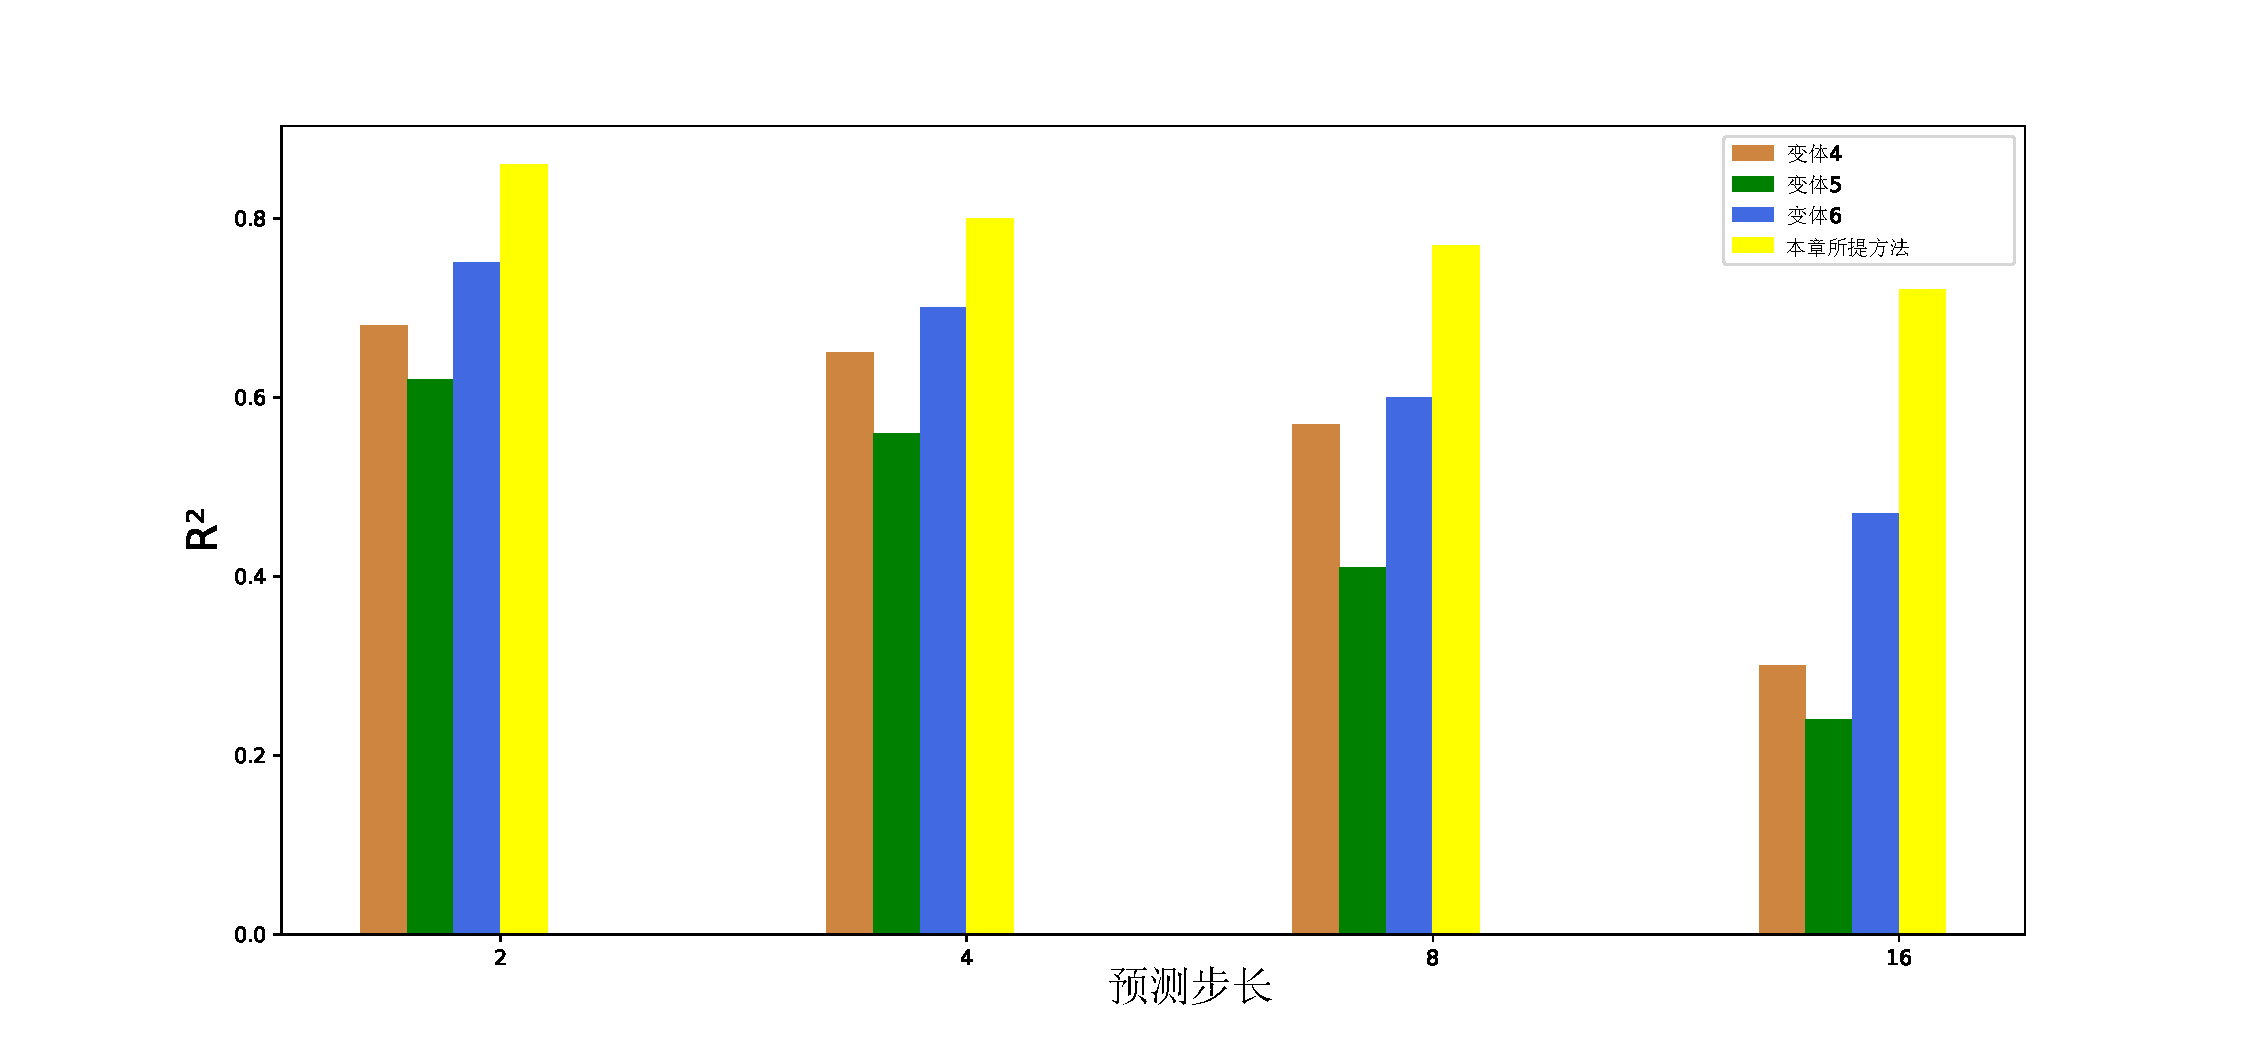
\includegraphics[scale=0.26]{./ch4/fig4_5.pdf}
\caption{变体(1-3)与本章所提出框架的消融实验性能比较。} \label{fig4_4}
\end{center}
\end{figure}

\begin{figure}[ht]
\begin{center}
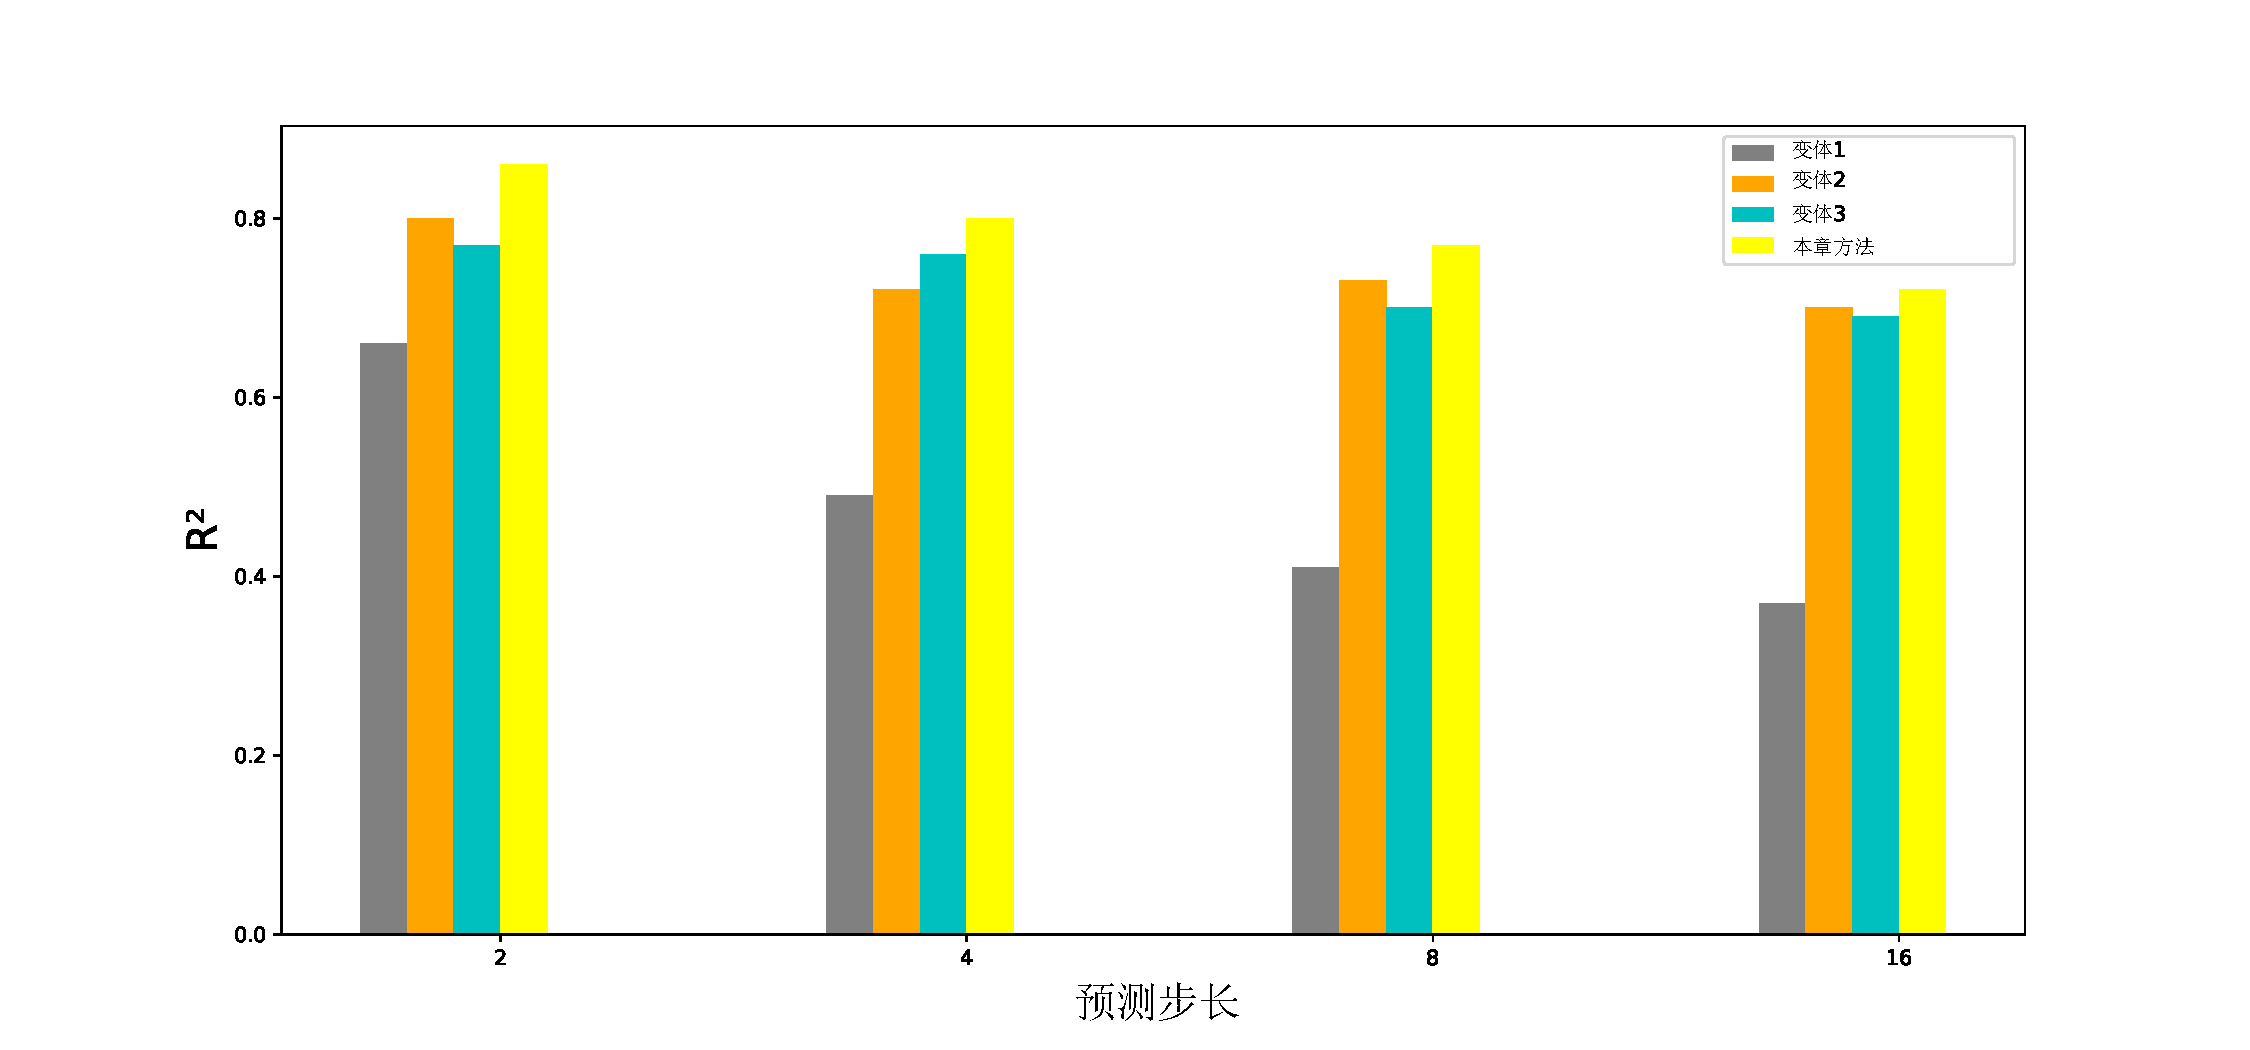
\includegraphics[scale=0.26]{./ch4/fig4_4.pdf}
\caption{变体(4-6)与本章所提出框架的消融实验性能比较。} \label{fig4_5}
\end{center}
\end{figure}

此外,在低频部分的基于混合注意力的预测模型中,混合注意力层由两部分组成:自我注意力层和时间注意力层。在这里,我们将进行进一步的实验和分析,以验证这两个部分的有效性。

自我注意层旨在增强模型捕捉长距离依赖关系的能力。如上文不同滑动窗口大小的实验结果所示,带有注意力机制的模型可以获得每个隐藏状态之间的全局相关性。注意分值的计算是自注意机制的核心步骤,为了进一步验证自注意层的有效性,我们对查询向量 $q$ 和关键向量 $k$ 之间的注意分值的不同计算方法的模型性能进行了研究。表\ref{table7}总结了不同技术水平的注意力向量的实验结果,包括余弦相似度(cosine similarity)\cite{AGraves2014}、MLP\cite{DBahdanau2014}、矩阵串联(matrix concatenation)和带权重的点积(dot product with weights),本文提出的模型采用了带权重的点积(dot product)。表\ref{table7}显示,本文采用的注意力向量以较少的计算量获得了最低的平均 MAE 和 RMSE。

最后,为了更好地理解时态注意层的有效性,我们在 STR1 路面数据集的实验中通过可视化图形显示对时态注意权重向量进行了分析。时间注意力向量的热图如图\ref{fig4_6}所示,热图中的每个网格代表注意力值,颜色越深,表示注意力值越高。注意力向量为 $\alpha \in \mathbb{R}^{l}$,其中 $l$ 等于前 LSTM 层生成的隐藏状态的维度,例如本实验中为 $l=24$。注意向量的值是每一行元素的相关性度量。参数越接近 0,相应位置特征对预测的贡献就越小。以在 STR1 数据上训练的时间模式注意力值为例,我们选取三个最高值,并追溯到隐藏状态 $h_{t} \in \mathbb{R}^{l}$ 在时间步长 $t$ 的相应位置上,滑动窗口大小为 5。这三个值对应的隐藏状态行元素分别为$[$ 0.1129, -0.4297, -0.1249, 0.2026, 0.04882$]$、$[$0.1125, -0.4264, -0.1050, 0.2278, 0.0524$]$和$[$0.1180, -0.4804, -0.1140, 0.2154, 0.0553$]$。显然,这三个行元素的分布是相似的。也就是说,这些位置上隐藏状态的行元素在与下一个隐藏状态 $h_{t}$ 连接时会做出更多贡献。

\begin{table}[h]
\centering
\caption{\label{table7}采用不同注意力权重计算方法的自我注意力层的性能}
\scalebox{0.92}{
\begin{tabular}{c c c c}
 \hline
  注意力机制 &  对应公式 & MAE & RMSE \\
 \hline
 dot product& $\alpha = exp(\frac{q \cdot k^{T}}{\sqrt{d_{k}}}) \// \sum^{T}_{\tau = 0} exp(\frac{Q_{\tau} \cdot K_{t}^{T}}{\sqrt{d_{k}}})$ & \textbf{0.55} & \textbf{0.81} \\
 \hline
  cosine similarity & $\alpha = \frac{q \cdot k^{T}}{\left \|q\right\| \cdot \left \|k\right\|}$ & 0.64 & 1.23 \\
 \hline
  concatenation & $\alpha = W[q;k]$ & 0.73 & 1.47 \\
 \hline
  MLP & $\alpha= \delta(W_{q}\cdot q + W_{k}\cdot k)$ & 0.57 & 0.85 \\
 \hline
 \end{tabular}}
\end{table}

\begin{figure}[htbp]
\begin{center}
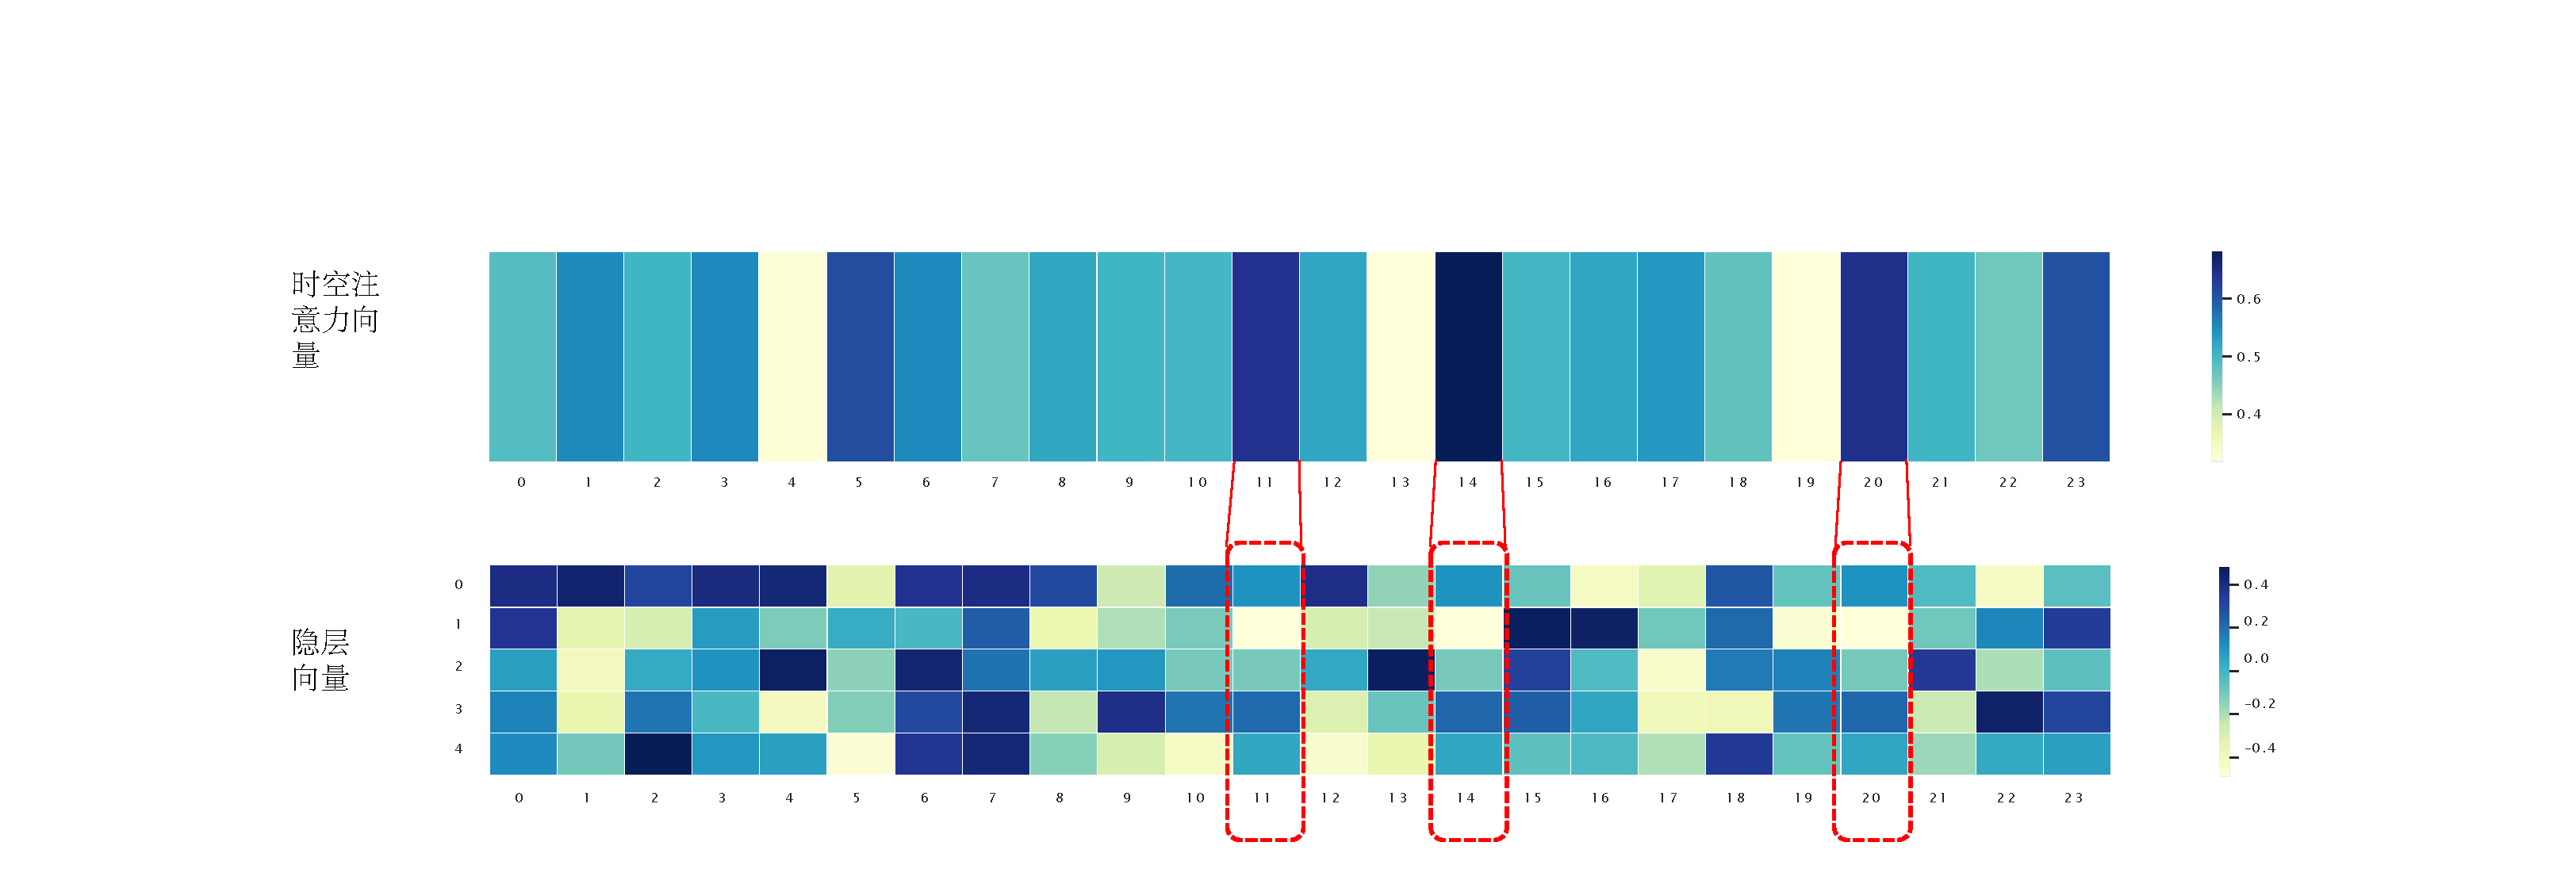
\includegraphics[scale=0.25]{./ch4/fig4_6.pdf}
\caption{时间注意力向量 $\alpha \in \mathbb{R}^{24 \times l}$ 和 5 个滑动窗口中的隐藏状态 $h \in \mathbb{R}^{5 \times 24}$ 可视化。前3个注意力值分别为 0.6396、0.6809 和 0.6421。} \label{fig4_6}
\end{center}
\end{figure}


\section{小结}

本章分析了分布式饱和脉冲控制下时滞复杂网络的局部动力学行为。首先,利用反证法、脉冲系统的比较原理和平均脉冲区间的方法研究了分布式饱和脉冲控制下具有耦合时滞的鲁里叶网络的局部指数同步问题,并给出了不依赖于时滞的基于 BMIs 的充分性判据。为了降低保守性,选取最新的具有更多松弛变量的改进凸包表示法来处理分布式饱和的脉冲项,并且开发了一种与收缩不变集完全不同的估计吸引域的方法。其次,通过构造依赖于脉冲时刻的复合型 Lyapunov 函数进一步降低保守性,讨论了分布式饱和脉冲控制下具有切换拓扑的非线性时滞多智能体系统的局部一致性,并建立了相应的局部一致性判据。为了估计出最大的吸引域,通过适当的矩阵变换,建立了基于 LMIs 的优化问题,并通过 Matlab 软件中的 Yalmip 工具箱求解相应的最大吸引域的数值解。  

本章部分结果已发表在国际期刊  IEEE Transactions on Neural Networks and Learning Systems 上,部分结果已投稿至国际期刊 IEEE
Transactions on Automatic Control。具体详见作者发表论文的清单。
